\chapter{Background}
\label{chp:background}

In this chapter we'll first discuss some technical aspect of video conferencing that affect how we reason about solving the challenges, before performing we try to benchmark existing solutions to see how they perform in our example conversations.

\section{WebRTC}

This thesis is largely inspired by the efforts of the \gls{w3c} in standardizing \gls{webrtc}, a technology which enables direct browser-to-browser communication. Building on \gls{webrtc}, services like Telenor Digital's appear.in and Telefonica's Hello have come to life, ushering in a new age of communication that does not depend on the traditional GSM infrastructure, but is fueled by faster Internet connections and more and more capable smartphones.

It's interesting to note that many of the largest WebRTC communication platforms (like appear.in and Hello, as mentioned) we've seen so far have been developed by the largest players in the traditional communication field, and not from any independent outsider. The big telephone companies do have capabilities other actors don't enjoy, such as being able to freely route calls back over GSM as a fallback solution in case a person is not reachable online, but this has not been a selling point for the services so far. The services have also largely been focused on video conferencing, even though the technology is equally well-suited for pure voice conversations or text-based communication.

In any case, the hard part of the problem is video conferencing, as the demands on the user equipement and connection is far greater than what will ever be excercised by voice or text. Group conversations on appear.in is today artificially limited to 8 people, but often the parties in the conversation will experience practical limits below this due to insufficient bandwidth or CPUs not capable of encoding enough parallel video streams.

The dynamic routing scheme proposed in this thesis is largely independent of underlying technology, but is intended to be built on top of \gls{webrtc}. The requirements to implement the suggested solution is that the platform allows clients to establish connections with a given starting bitrate (which WebRTC allows through modifying the SDP offer), and that streams can be routed arbitrarily. As connections have to be established in an ad-hoc way out-of-band in WebRTC, as long as the parties involved all share session keys, this should also be feasible.


\section{A Technical Look at Video Conferencing}

\subsection{Hardware}

\todo{Write about what hardware performs encoding. CPU for VP8, hardware-accel for H264, GPU potential, custom machinery (ala cisco)}


\subsection{CPU limitations}

The naïve approach to encoding video is to encode the raw stream from the web camera into several client-optimized streams for transmission. Using VP8, this is the only way to do it. However, H.264 can be encoded in a \gls{svc} manner, which makes it possible to extract different bandwidth-streams from a single stream. With VP8 this is sadly not possible, and the only alternative is to utilize a \gls{sfu}, a technique where several streams are sent to the same endpoint, which can then select which of the streams to forward to the different endpoints. This is not as efficient as sending only a single stream however, and the encoding step is also costlier on the CPU.


\subsection{Continuous Presence vs. VAS}

There are mainly two different ways to do video conferencing, Continuous presence and \gls{vas}. Continuous presence means that all parties in the conversation is visible to all other parties at the same time. \gls{vas} means that

The \autoref{fig:service-possibilities} summarizes the possible services that can be provided for different amounts of available bandwidth. A minimal video unit is the smallest bitrate it makes sense to encode video in. This will be service dependent, but we can imagine a number around $\approx$500kbps will be reasonable.

\begin{figure}
    \centering
    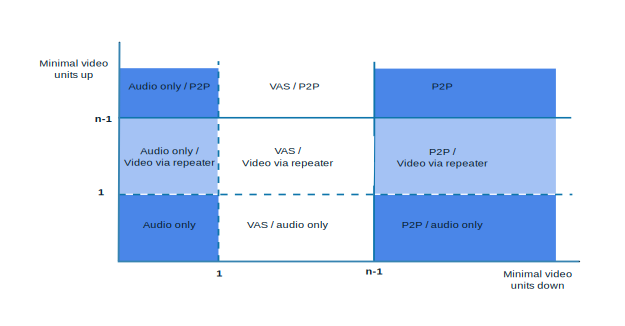
\includegraphics[width=\textwidth]{commcap}
    \caption{The possible services for different upload/download bandwidths. A minimal video is the smallest bitrate where it makes sense to send video. Dark blue is what appear.in can provide today (audio only requires manual configuration), light blue is what's possible with the solution suggested later in this thesis.}
    \label{fig:service-possibilities}
\end{figure}


\todo[inline]{Only do Continous Presence if the client has enough available bandwidth, ie $BW_{down}>(n-1)*BW_{min}$, otherwise fall back to \gls{vas} through an \gls{mcu}}

\todo[inline]{Write about Continuous Presence (multiple parties on-screen at the same time), and how that limits the different topologies}


\section{The current providers}

A selection of widely-known video conferencing solutions today, with significantly different network architectures are summarized in the following table.

\begin{center}
	\label{tab:existing-solutions}
	\begin{tabular}{| l | l |}
		\hline
		\textbf{Service} & \textbf{Description} \\ \hline
		appear.in & Peer-to-peer WebRTC service \\ \hline
		Google Hangouts & Browser-based service utilizing a Google MCU \\ \hline
		Microsoft Skype & Downloadable app, closed source protocol \\ \hline
		Cisco TelePresence & Custom hardware, self-hosted or cloud service \\ \hline
	\end{tabular}
\end{center}

Notably absent here is FaceTime, Apple's videochat service bundled with their devices. FaceTime's absence in this thesis is due to the lack of support for more than two people in a conversation, which makes the optimal topology question embarassingly easy to answer, and the lack of support on non-Apple devices, which makes the service uninteresting to us.

We also note that Mozilla just entered the market in collaboration with Telefonica with their Hello service, bundled with recent versions of Firefox\footnote{https://www.mozilla.org/en-US/firefox/hello/}. Hello however essentially provides the same service as appear.in, just bundled with the browser. Thus anything we say about appear.in applies to Firefox Hello as well (and all other peer-to-peer WebRTC services), and we'll therefore not consider them separately. This author will however congratulate Mozilla and Telefonica on their endeavor to make communication more open and available to anyone.

Let's take a more detailed look at these services.

\subsection{appear.in}

appear.in is a free peer-to-peer service built on WebRTC that does not require sign-ups or installation of addons to your browser. Due to the WebRTC requirement the service is available to anyone using a recent version of either Google Chrome, Mozilla Firefox or Opera, while the OS-provided browsers (Internet Explorer and Safari) have notably not implemented WebRTC yet.

\todo[inline]{Write a bit more about appear.in architecture: linear scaling, contionus presence, ease of testing due to no signups, limit of 8 people}


\subsection{Google Hangouts}

Google Hangouts is alongside appear.in the only other service based in the browser. Hangouts is a merge of several earlier Google communication solutions like Google Talk, Google+ Messenger and the Hangouts feature from Google+. The service uses a Google-provided \gls{mcu}, and VP8/9 over WebRTC as video transport\todo{Find a source to verify this}. A conversation is limited to 10 people.

To use Google Hangouts it requires you to setup a public Google+ profile, which makes the barrier of entry significantly higher than for some of the other services tested in this thesis. It also requires installing the Hangouts extension for video conferencing to work. Since you cannot do video hangouts with yourself, this necessitates managing as many Google accounts as you need nodes in your conversation, and call management is a true \gls{pita} compared to the simplicity of appear.in, where creating or joining a conversation is a simple matter of visiting a URL.


\subsection{Skype}

Skype is probably the most well-known of the solutions we're looking at, being among the first to offer free video conferencing for personal use. Skype was also among the first to provide a VoIP solution interoperating with \gls{pstn}, easing the barrier of entry for new users. The original Skype topology was peer-to-peer, routing streams through PCs with Skype installed that had the app running, using a proprietary closed-source protocol. After the Microsoft aquisition Skype ditched the peer-to-peer design to a Microsoft MCU-backed solution, justified as a means to improve performance and security for users. A Skype conversation has a soft limit on five people for the best user experience, hard limited to 10 users.

Skype requires a standalone application to run, which is available on pretty much every platform out there, including Windows, Mac, Linux, Android, iOS, Windows Phone, BlackBerry, most tablets, TVs, gaming consoles and more. The benefit is close access to hardware and GPUs for more efficient video encoding, the downside is the lack of open protocols, standardization and transparency.


\subsection{Cisco}

\todo{Write about Cisco}

\subsection{Performance Summary}

The following table summarizes where the limits for each provider is at the moment.

\todo[inline]{Add performance chart as where providers fit on a bwup/bwdown spectrum}


\section{Test Cases}

To narrow down the problem scope a little, we'll define some example conversations we can work on, and assume that if we can efficiently serve these setups, we can serve most others as well. A summary of the test cases are given in \autoref{tab:example-conversations}. Note that these are intended to be hard cases, with at least one node being more constrained than the others. \autoref{fig:test-cases} illustrates the test cases graphically with the all the inter-node latencies.

\begin{center}
    \captionof{table}{Test Cases}
    \label{tab:example-conversations}
    \begin{tabular}{| l | l | p{7cm} |}
    \hline
    \textbf{Case name} & \textbf{$n$} & \textbf{Description} \\ \hline
    Traveller & 3 & Two people with decent connections between them, one remote with high latency and severely restricted bandwidth to the others. \\ \hline
    Standup & 4 & Two people on desktop machines with wired connections, one laptop and one tablet on wifi. \\ \hline
    Friends & 7 & Group split in two locations, each subgroup having short latencies internally, but larger latencies to the other group. Heterogenous bandwidths across the board. \\ \hline
    \end{tabular}
\end{center}

Are there any trivial cases we can ignore? As long as there's only two people in a conversation, and they have fairly low latency between each other and sufficient bandwidth, peer-to-peer is the optimal choice in all cases. Initially, it might seem like this would indeed be the case in all conversations with two participants, and not just the good-bandwidth, small-latency onces. However, this is not the case. To illustrate why, consider a conversation between two people, one in Europe and one in Asia. The latency between them is ~350ms. They both have fairly acceptable bandwidth, with 3Mbps each, which should be plenty to sustain an acceptable video link between them. This, however, is not the case, as the bandwidth between them is far more limited due to the long distance and many hops through publicly routed networks. However, each of the peers has a datacenter of a distributed VPS provider nearby, to which they can utilize their full bandwidth. And these distributed VPS providers tend to have established high-quality routes between their own datacenters, backed by \glspl{sla} and with all the bells and whistles you don't get on your private Internet connection.

The available bandwidth between the two datacenters is thus far greater than what can be achieved directly between the two peers. Because of this, their video link can be improved by routing their traffic through the datacenters, thus enabling each peer to utilize the full bandwidth of their connection.\footnote{This is backed by a simple experiment, using DigitalOcean as our VPS provider. From a 100Mbit university connection in Norway, sustained datarates to their Singapore datacenter varied greatly, measuring 90kBps, 3,7MBps, 1,9MBps and 2,58MBps for each test. However, from their Amsterdam datacenter, a consistent throughput of 24,6MBps was measured} Do however note that the latency is close to unchanged from routing through the datacenters, only sustained bandwidth between the peers is improved (and probably packet loss).

These conversations are not extensive, but should cover enough corner cases to be able to highlight the pros and cons of the different topologies. The examples cover the low-latency, few peers conversations; the bandwidth-challenged cases; the high-latency conversations; and the very hetrogenous device conversations, where one or more party is severly challenged in terms of either bandwidth or latency.

We assume that the backend networks are not saturated, and that each user is bandwidth-constrained only by their connection. By extension, the maximum bandwidth attainable between any pair of nodes in our network is the lesser of the upload bandwidth of the sending party and the download bandwidth of the receiving party. However, latency has to be defined for any pair of the nodes in the network, as this is mostly determined by their geographical location in relation to each other. To best illustrate the physical topology, we can draw each scenario as a complete graph:

\begin{figure}
    \begin{subfigure}{\textwidth}
        \centering
        \digraph{exampleconvchat}{
            edge [dir=none];
            rankdir=LR;
            a [label="A (20/5)"];
            b [label="B (30/15)"];

            a -> b [label="8ms"];
        }
        \subcaption{Example conversation ``traveller''.}\label{fig:example-conv-chat}
    \end{subfigure}

    \begin{subfigure}{\textwidth}
        \centering
        \digraph{exampleconvcasual}{
            edge [dir=none];
            rankdir=LR;
            a [label="A (10/2)"];
            b [label="B (30/5)"];
            c [label="C (2/1)"];

            a -> b [label="5ms"];
            a -> c [label="10ms"];
            b -> c [label="15ms"];
        }
        \caption{Example conversation ``standup''}\label{fig:example-conv-casual}
    \end{subfigure}

    \begin{subfigure}{\textwidth}
        \centering
        \digraph{exampleconvbusiness}{
            edge [dir=none];
            a [label="A (50/50)"];
            b [label="B (50/50)"];
            c [label="C (50/50)"];
            d [label="D (30/30)"];

            a -> b [label="2ms"];
            a -> c [label="2ms"];
            a -> d [label="150ms"];
            b -> c [label="2ms"];
            b -> d [label="150ms"];
            c -> d [label="150ms"];

            {rank=same; a b}
            {rank=same; c d}
        }
        \caption{Example conversation ``friends''}\label{fig:example-conv-business}
    \end{subfigure}
    \caption{The different test cases}
    \label{fig:test-cases}
\end{figure}
\todo{Make actual test cases}
